\chapter{Hardware design flow on FPGA}

Now that the reader is aware of the internal structure of FPGAs, the design flow on these FPGAs can 
be discussed. Indeed, a series of more or less compulsory steps are required to carry out the 
design of an embedded system on FPGA. This chapter is dedicated to the description of this 
design flow and the tools used to carry it out. All the tools that are discussed in this chapter are
part of a super-tool named Quartus. Quartus is the main software used for the development on Intel 
FPGA. In fact, it is a kind of IDE for hardware development. It interfaces many tools together to
ease the work of the users.

\section{Design flow}

The very first step is of course to choose an FPGA, once this is done, one must start by assigning 
the inputs and outputs of the FPGA. This step is named I/O Planing in Figure \ref{fig:flow/design_flow}.

\begin{figure}[ht]
    \centering
    \includegraphics[scale=0.5]{Chapter2-FPGA_Flow/res/blockdiagram-quartus-flow.png}
    \caption{Intel FPGA design flow on Quartus}
    \label{fig:flow/design_flow}
\end{figure}

\subsection{I/O Planning}

During this I/O Planing step, the user has to choose which input or output of his design goes to 
which physical input or output of the FPGA. It is also during this step that the types of I/Os, the 
standards they should use etc. are set. In the context of this work, this step could be skipped. 
Indeed, the manufacturer of the DE10-Nano board provides with its board a Quartus project 
containing the definition of the I/Os in order to correspond to what is present on the board. 
This greatly simplifies the task and avoids digging through all the datasheets of the different
components of the board to find out how to set up all the IOs.

\subsection{Design Entry}

In this step, the user defines the different logical entities that are needed to build up the 
desired circuit. A logical entity or a module is simply a sub-circuit with a given interface, an
example is shown later in this section.

All this is done in a so-called hardware description language. There is no need for special tools 
here, a simple text editor will do. However, Quartus contains an editor that can be used for this 
purpose. Concerning the languages, there is a multitude of choices. But there are three frequently used 
languages. These are VHDL, Verilog and System Verilog. VHDL is a high level language that is highly typed.
Verilog and System Verilog are weakly typed and of lower level. For example, in VHDL it is 
frequent to work directly on data-structures, complex types that can quickly hide the logic of an 
architecture. In Verilog and System Verilog, few types are provided and the hardware architect does 
regularly work with registers and words in which the bits are assignable one by one. Since System 
Verilog is a newer language and not always (correctly) supported by the tools, it was decided to use 
Verilog for this work. 

It should be noted that these languages, although similar to software programming languages, do not 
work in the same way. Indeed, in a Verilog file for example, one defines what is called a module. 
This module has inputs and outputs. Each input and output can either be defined as a wire, 
which means that this I/O have no specific functionality, it just serves as a connection, or 
as a reg, which means that this I/O is registered. A register is therefore placed at this I/O. 

Inside the module, the developer then defines how these inputs and outputs are linked. Here again, 
two possibilities are available to the user. Indeed, it is possible to define circuits that are 
either combinatorial or sequential. For the combinatorial circuits, they can take any input 
(registered or not) and transmit its outputs to non-registered outputs. It is important that the 
output is non-registered because combinatorial circuits are asynchronous, the compiler would not 
understand who is driving the register if it was put directly at the output of a combinatorial 
circuit. The other possibility is to describe sequential circuits. For these, a sensitivity list 
must be chosen. That is to say, signals that have the effect of updating the circuit. In 
general, only the clock is used, and the state of the circuit changes at each clock cycle. Note that
any other signal specified in that list might result in an asynchronous response of the circuit, as
the circuit responses to a clock change and also to a change of this signal. This is useful to
implement asynchronous resets in synchronous circuits. Sequential circuits can take registered or
not inputs but can only transmit their output to registers. It should be noted that a combinatorial 
circuit and a sequential circuit can be cascaded since sequential circuits accept non-registered 
inputs. This makes it possible to put a combinatorial output on an output register for example, even
though it is impossible with the combinational circuit alone. 

At the level of sequential circuits, another subtlety compared to software programming languages 
should be noted. The assignment of registers is done in a blocking way. This means that these 
assignments are only effective at the next clock cycle (or next sensitivity signal update) and 
that all these assignments are made at the same time in parallel. One should not forget that the 
language describes circuits. And so all outputs appear at the same time once the rising or falling 
edge of the clock is perceived. For example assigning x to a and then a to b results in
a[t] containing x[t - 1] and b[t] contains a[t - 1], which might not be obvious for a software
developer.

All this is a lot of information, so a small example of a module described in Verilog is given 
below. This one simply describes an AND logic gate whose output is registered. The corresponding 
circuit is shown in Figure \ref{fig:verilog/register_and}.

\begin{lstlisting}[language=Verilog, caption=Verilog Registered AND gate example]
module registered_and(
    clk,
    input0,
    input1,
    output0
);

// clk is defined as an input wire 
input wire clk;   
// input0 is defined as an input wire  
input wire input0;  
// input1 is defined as an input wire
input wire input1; 
// output0 is defined as an output and it is registered
output reg output0; 


// An internal wire is defined
wire and_output;    

// Describes an and gate between input0 and input1
// and put the result on the wire and_output asynchronously
assign and_output = input0 & input1; 

// Sequential circuit that updates at rising edge of clk
always @(posedge(clk)) begin
    // The circuit simply directs the value present on "and_output" at 
    // that moment to the registered output (ie, it sets the register).
    output0 <= and_output;                      
end

endmodule

\end{lstlisting}

\begin{figure}[H]
    \centering
    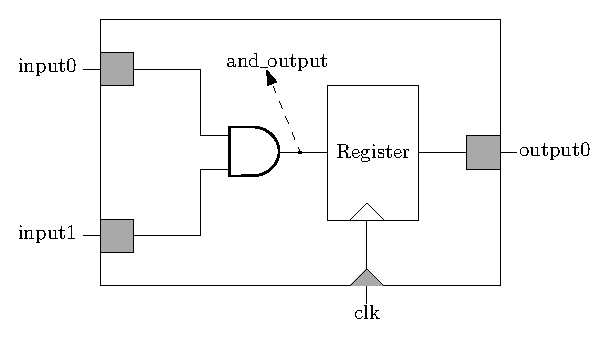
\includegraphics[scale=1.0]{Chapter2-FPGA_Flow/res/register_and}
    \caption{Intel FPGA design flow on Quartus}
    \label{fig:verilog/register_and}
\end{figure}

Other tools than programming allow to define modules. A particularly useful tool is the IP creation 
Mega Wizard shown in Figure \ref{fig:tools/megawizard}. This tool allows the user to create some common 
blocks such as on-chip RAMs using a graphical interface where one can choose the different options. 
For a RAM the user can choose the word size, the number of words, whether the memory has 
two ports or not, etc. At the end of the configuration, the wizard generates the Verilog file 
describing the module just defined.

\begin{figure}[H]
    \centering
    \includegraphics[scale=0.6]{Chapter2-FPGA_Flow/res/megawizard.PNG}
    \caption{IP creation Mega Wizard window}
    \label{fig:tools/megawizard}
\end{figure}

\subsection{Interconnect Design Entry}

This step is equivalent to the simple design entry, i.e. the goal is to describe the architecture. 
However, as the tool to design the interconnect is specific, a section is dedicated to it. As seen 
before the interconnect is the part of the architecture that links the two parts: FPGA and ARM. The 
use of the buses is done through several signals, which can quickly be annoying and complicated to 
maintain directly through the verilog files. The tool of this step which is Qsys allows to link 
the masters and slaves of the FPGA to those of the ARM processor in a graphic interface. In this 
tool, the address space of each slave has to be specified. Qsys checks if the specified 
addresses are not outside the address space of the master to which they are connected. Figure \ref{fig:tools/qsys} 
shows the interface to the HPS (ARM processor) and the connections to a slave.

In addition to the signals that are useful for communication on the interconnect, others allow interraction 
with the FPGA. This means that these signals are inputs or outpus of the Verilog that is generated
by QSys. They can thus be connected to other circuits on the FPGA side, contrary to the other
signals shown in QSys. These signals ared called exported signals and the user can chose which one
is exported, usualy the ones that are not direct links of the interconnect. Once a system is 
described, it only
remains to ask Qsys to generate the system. It then creates all the necessary Verilog files that 
can be used as a single module later in the user's Verilog code. This module receives as inputs and 
outputs all the signals that have been exported. To summarize, QSys is a kind of graphical 
programming software.

\begin{figure}[H]
    \centering
    \includegraphics[width=\linewidth]{Chapter2-FPGA_Flow/res/qsys.PNG}
    \caption{QSys window with an HPS named hps\_0 and a slave module named mm\_bus}
    \label{fig:tools/qsys}
\end{figure}

In Figure \ref{fig:tools/qsys} different elements have been highlighted. The two entities present in the system are 
represented in yellow, there is thus the HPS named hps\_0 which is an external representation of the 
ARM processor and an Avalon to External Bus Bridge called im\_bus which makes it possible to make 
the link between a bus of the interconnection and a bus defined by the user on the FPGA. This module 
is discussed again later. In each module, some lines are in red. Red represents the 
different slaves of the system. In the base and end columns, it can be seen that these slaves have 
a defined address space. They all start at 0 because they are relative to the starting address of 
the master. In green, in the im\_bus can be seen an exported signal, this one is accessible 
from the FPGA. In fact, most of the lines shown in QSys represent several signals describing entities,
 bus, ... Finally, a master-slave connection is shown in blue.

\subsection{Simulation}

Once the different modules of the system have been defined, it can be interesting to simulate some 
of them. This step is not necessarily mandatory but it can save a lot of time if the system is big. 
Indeed, compiling a large system can quickly take several hours, or days. The verifications are 
therefore done before compilation by simulation and not afterwards by measurements on the working 
system. 
Sometimes, the simulation is also more practical because it allows to easily generate precise 
scenarios. To simulate, the tool used by quartus is Modelsim. In this tool, signals can be fixed 
and tests can be performed. All signals are then displayed so that the user can verify the 
behavior.

\subsection{Synthesis and Fitter}

These two steps are the first of the compilation. The compiler transforms the descriptions made
 in verilog into a logic circuit and then try to fit everything on the FPGA used. It checks that 
 the resources are sufficient for the described design. The whole fitting process is 
 time-constrained. This means that it places the different blocks in such a way that the delays 
 are minimal. After the Synthesis, the user can display the circuit to verify parts of its design
 visually. The tool used for this is the RTL net viewer. An example is given in Figure 
 \ref{fig:tools/rtl}.

 \begin{figure}[H]
    \centering
    \includegraphics[width=\linewidth]{Chapter2-FPGA_Flow/res/rtl.PNG}
    \caption{The beta machine CPU high level view in RTL viewer}
    \label{fig:tools/rtl}
\end{figure}

\subsection{Timing Analysis and Design Optimal}

FPGA designs are totally dictated by time constraints. The purpose of this step is to check if the 
constraints are well respected by the design, after fitting. All this is done by simulation by 
testing the signal propagation delays at different temperatures. If one of the tests fails, the 
design is not validated and it has to be modified. For a timing to be validated, it is 
necessary for example that all the stages of a circuit have finished their work in the time existing 
between two rising edges of the clock. The software responsible for these verifications (TimeQuest) 
does a lot of tests and measurements but these are not discussed in this work, this is outside of the 
scope. What is important to remember is that the user sets the constraints, by imposing the clock 
frequencies and so on and the software then takes care of checking them in the worst possible 
scenarios. 

\subsection{On-Chip Debug}

The last step is to program the FPGA with the just compiled and timing-validated design. This is done
using the Quartus Programmer, it is a straight forward manipulatin and there is not much to say
about it. Nevertheless, one still has to perform a last verification, the one in real environment. 
Most of the time, it is errors made during the Design Entry that are seen here. For 
example, the user has connected components incorrectly, in a way that is not structurally 
wrong but is functionally wrong. Other errors that are not totally due to the user can also occur 
but are very specific (e.g. bugs due to operations on clock signals, ...).

To help the user in this debugging task, a really handy tool is provided in the Intel suite. This 
tool is the Signal Tap Logic Analyzer. Indeed, it allows to add a logic analyzer to the design 
which is connected to signals of the design that the user can choose. If the design and the 
analyzer are present on the FPGA, it is possible to display the signals in real time in the tool 
window when the board is connected to the computer. This tool also allows to make more advanced 
measurements such as triggered measurement which launches the recording of the data when a given
trigger occures (when a signal goes high for example). In short, it is the perfect tool for debugging.